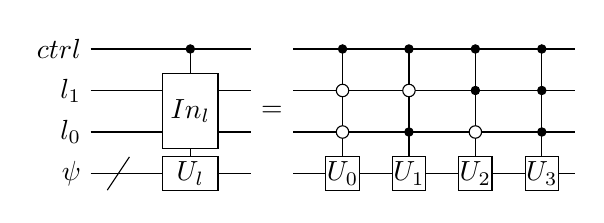
\begin{tikzpicture}[scale=1.000000,x=1pt,y=1pt]
\filldraw[color=white] (0.000000, -7.500000) rectangle (175.000000, 52.500000);
% Drawing wires
% Line 1: ctrl W ctrl
\draw[color=black] (0.000000,45.000000) -- (175.000000,45.000000);
\draw[color=black] (0.000000,45.000000) node[left] {$ctrl$};
% Line 2: l1 W l_1
\draw[color=black] (0.000000,30.000000) -- (175.000000,30.000000);
\draw[color=black] (0.000000,30.000000) node[left] {$l_1$};
% Line 3: l0 W l_0
\draw[color=black] (0.000000,15.000000) -- (175.000000,15.000000);
\draw[color=black] (0.000000,15.000000) node[left] {$l_0$};
% Line 4: sys W \psi
\draw[color=black] (0.000000,0.000000) -- (175.000000,0.000000);
\draw[color=black] (0.000000,0.000000) node[left] {$\psi$};
% Done with wires; drawing gates
% Line 6: sys /
\draw (6.000000, -6.000000) -- (14.000000, 6.000000);
% Line 8: l0 l1 G width=20  $In_l$ sys G width=20 $U_l$ ctrl
\draw (36.000000,45.000000) -- (36.000000,0.000000);
\begin{scope}
\draw[fill=white] (36.000000, 22.500000) +(-45.000000:14.142136pt and 19.091883pt) -- +(45.000000:14.142136pt and 19.091883pt) -- +(135.000000:14.142136pt and 19.091883pt) -- +(225.000000:14.142136pt and 19.091883pt) -- cycle;
\clip (36.000000, 22.500000) +(-45.000000:14.142136pt and 19.091883pt) -- +(45.000000:14.142136pt and 19.091883pt) -- +(135.000000:14.142136pt and 19.091883pt) -- +(225.000000:14.142136pt and 19.091883pt) -- cycle;
\draw (36.000000, 22.500000) node {$In_l$};
\end{scope}
\begin{scope}
\draw[fill=white] (36.000000, -0.000000) +(-45.000000:14.142136pt and 8.485281pt) -- +(45.000000:14.142136pt and 8.485281pt) -- +(135.000000:14.142136pt and 8.485281pt) -- +(225.000000:14.142136pt and 8.485281pt) -- cycle;
\clip (36.000000, -0.000000) +(-45.000000:14.142136pt and 8.485281pt) -- +(45.000000:14.142136pt and 8.485281pt) -- +(135.000000:14.142136pt and 8.485281pt) -- +(225.000000:14.142136pt and 8.485281pt) -- cycle;
\draw (36.000000, -0.000000) node {$U_l$};
\end{scope}
\filldraw (36.000000, 45.000000) circle(1.500000pt);
% Line 10: =
\draw[fill=white,color=white] (58.000000, -6.000000) rectangle (73.000000, 51.000000);
\draw (65.500000, 22.500000) node {$=$};
% Line 12: sys G $U_0$ -l0 -l1 ctrl
\draw (91.000000,45.000000) -- (91.000000,0.000000);
\begin{scope}
\draw[fill=white] (91.000000, -0.000000) +(-45.000000:8.485281pt and 8.485281pt) -- +(45.000000:8.485281pt and 8.485281pt) -- +(135.000000:8.485281pt and 8.485281pt) -- +(225.000000:8.485281pt and 8.485281pt) -- cycle;
\clip (91.000000, -0.000000) +(-45.000000:8.485281pt and 8.485281pt) -- +(45.000000:8.485281pt and 8.485281pt) -- +(135.000000:8.485281pt and 8.485281pt) -- +(225.000000:8.485281pt and 8.485281pt) -- cycle;
\draw (91.000000, -0.000000) node {$U_0$};
\end{scope}
\draw[fill=white] (91.000000, 15.000000) circle(2.250000pt);
\draw[fill=white] (91.000000, 30.000000) circle(2.250000pt);
\filldraw (91.000000, 45.000000) circle(1.500000pt);
% Line 13: sys G $U_1$ l0 -l1 ctrl
\draw (115.000000,45.000000) -- (115.000000,0.000000);
\begin{scope}
\draw[fill=white] (115.000000, -0.000000) +(-45.000000:8.485281pt and 8.485281pt) -- +(45.000000:8.485281pt and 8.485281pt) -- +(135.000000:8.485281pt and 8.485281pt) -- +(225.000000:8.485281pt and 8.485281pt) -- cycle;
\clip (115.000000, -0.000000) +(-45.000000:8.485281pt and 8.485281pt) -- +(45.000000:8.485281pt and 8.485281pt) -- +(135.000000:8.485281pt and 8.485281pt) -- +(225.000000:8.485281pt and 8.485281pt) -- cycle;
\draw (115.000000, -0.000000) node {$U_1$};
\end{scope}
\filldraw (115.000000, 15.000000) circle(1.500000pt);
\draw[fill=white] (115.000000, 30.000000) circle(2.250000pt);
\filldraw (115.000000, 45.000000) circle(1.500000pt);
% Line 14: sys G $U_2$ -l0 l1 ctrl
\draw (139.000000,45.000000) -- (139.000000,0.000000);
\begin{scope}
\draw[fill=white] (139.000000, -0.000000) +(-45.000000:8.485281pt and 8.485281pt) -- +(45.000000:8.485281pt and 8.485281pt) -- +(135.000000:8.485281pt and 8.485281pt) -- +(225.000000:8.485281pt and 8.485281pt) -- cycle;
\clip (139.000000, -0.000000) +(-45.000000:8.485281pt and 8.485281pt) -- +(45.000000:8.485281pt and 8.485281pt) -- +(135.000000:8.485281pt and 8.485281pt) -- +(225.000000:8.485281pt and 8.485281pt) -- cycle;
\draw (139.000000, -0.000000) node {$U_2$};
\end{scope}
\draw[fill=white] (139.000000, 15.000000) circle(2.250000pt);
\filldraw (139.000000, 30.000000) circle(1.500000pt);
\filldraw (139.000000, 45.000000) circle(1.500000pt);
% Line 15: sys G $U_3$ l0 l1 ctrl
\draw (163.000000,45.000000) -- (163.000000,0.000000);
\begin{scope}
\draw[fill=white] (163.000000, -0.000000) +(-45.000000:8.485281pt and 8.485281pt) -- +(45.000000:8.485281pt and 8.485281pt) -- +(135.000000:8.485281pt and 8.485281pt) -- +(225.000000:8.485281pt and 8.485281pt) -- cycle;
\clip (163.000000, -0.000000) +(-45.000000:8.485281pt and 8.485281pt) -- +(45.000000:8.485281pt and 8.485281pt) -- +(135.000000:8.485281pt and 8.485281pt) -- +(225.000000:8.485281pt and 8.485281pt) -- cycle;
\draw (163.000000, -0.000000) node {$U_3$};
\end{scope}
\filldraw (163.000000, 15.000000) circle(1.500000pt);
\filldraw (163.000000, 30.000000) circle(1.500000pt);
\filldraw (163.000000, 45.000000) circle(1.500000pt);
% Done with gates; drawing ending labels
% Done with ending labels; drawing cut lines and comments
% Done with comments
\end{tikzpicture}
